In this section, we demonstrate that the interpolation points can also be
selected from a Voronoi tessellation procedure. For a $d$-dimensional space, the
Voronoi tessellation partitions a set of points $\{\Br_{i}\}_{i=1}^{N_{g}}$ in
$\BBR^{d}$ into a number of disjoint cells. The partition is based on the
distance of each point to a finite set of points, called its generators. In our
context, let $\{\Brhat_\mu\}_{\mu=1}^{N_{\mu}}$ denote such a set of generators,
and the corresponding cell, $\calC_\mu$, of a given generator $\Brhat_\mu$ is
defined as a cluster of points
\begin{equation}\label{eqn:vcell}
  \calC_\mu = \{\Br_{i} ~\vert~\dist(\Br_{i}\,,\, \Brhat_\mu) <
  \dist(\Br_{i}\, ,\, \Brhat_\nu) \textrm{ for all } \nu \neq \mu\}.
\end{equation}
The distance can be chosen to be any metric, e.g. the $L_2$ distance as $\dist
(\Br\,,\,\Br')=\norm{\Br-\Br'}_2$. In the case when the distances of a point
$\Br$ to $\Brhat_\mu, \Brhat_\nu$ are exactly the same, we may arbitrarily
assign $\Br$ to one of the clusters.

The Centroidal Voronoi tessellation (CVT) is a specific type of Voronoi
tessellation in which the generator $\Brhat_\mu$ is chosen to be the centroid of
its cell. Given a weight function $\rho(\Br)$ (such as the electron density),
the centroid of a cluster $\calC_\mu$ is defined as
\begin{equation}\label{eqn:centcomp}
  \Bc(\calC_\mu) = \frac{\sum_{\Br_{j}\In \calC_\mu} \Br_j\;\rho
  (\Br_j)}{\sum_{\Br_j\In \calC_\mu}\rho(\Br_j)}.
\end{equation}
Combined with the $L_2$ distance, CVT can be viewed as a minimization problem
over both all possible partition of the cells and the centroids as \cite{MacQueen1967}
\begin{equation}\label{eqn:CVT}
  \{\calC_\mu^\ast,\Bc_{\mu}^{*}\} = \argmin_{\{\calC_\mu, \Bc_{\mu}\}} \sum_
  {\mu=1}^{N_{\mu}} \sum_{\Br_k\in \calC_\mu}\rho(\Br_k)\norm{\Br_i-\Bc_{\mu}}^2,
\end{equation}
and the interpolation points are then chosen to be the minimizers
$\Brhat_\mu=\Bc_{\mu}(\calC_\mu^\ast)=\Bc_{\mu}^{\ast}$. Following the
discussion in \S \ref{cvtsec:int}, the electron density as the weight function~
\eqref{eqn:CVT} enforces that the interpolation points should locate at points
where the electron density is significant and hence satisfies the requirement 
(1). Since the cells $\calC_\mu^\ast$ are disjoint, the centroids $\Bc_{\mu}^
\ast$ are also separated by a finite distance away from each other and hence
satisfies the requirement (2). Because the ISDF decomposition is a highly
nonlinear process, in general we cannot expect the choice of interpolation
points from CVT decomposition to maximally reduce the error of the
decomposition. Instead, we demonstrate that the choice of the interpolation
points from CVT approximately minimizes the residual for the ISDF decomposition,
and hence provides a heuristic solution to the problem of finding interpolation
points.

\begin{theorem}
  When the set of electron orbitals $\{\varphi_i\}$ are Lipschitz continuous,
  CVT method approximately minimizes the residual error of the ISDF
  decomposition.
\end{theorem}
\begin{proof}
  For simplicity we assume the limiting case where $\varphi_{i}=\psi_{i}$, and
  hence each row of $\BZ$ is $\BZ(\Br)=[\varphi_{i}(\Br)\varphi_{j}(\Br)]_
  {i,j=1}^N$.

  Now suppose we cluster all matrix rows of $\BZ$ into sub-collections $
  \{\calC_\mu\}_{\mu=1}^{N_\mu}$, and for each $\calC_\mu$ we choose a
  representative matrix row $\BZ(\Br_\mu)$. Then the error of the ISDF can be
  approximately characterized as
  \begin{equation}\label{eqn:ISDFerror}
    R = \sum_{\mu = 1}^{N_\mu}\sum_{\Br_k\In \calC_\mu}\norm{\BZ(\Br_k)-
    \Proj_{\Span\{\BZ(\Br_{\mu})\}}\BZ(\Br_k)}^2,
  \end{equation}
  where the projection is defined according to the $L_2$ inner product as
  \begin{equation}\label{eqn:Zprojection}
    \Proj_{\Span\{\BZ(\Br_{\mu})\}}\BZ(\Br_k) = \frac{\BZ(\Br_{k})\cdot \BZ
    (\Br_\mu)}{\BZ(\Br_\mu)\cdot \BZ(\Br_\mu)}\BZ(\Br_{\mu}).
  \end{equation}
  Let $\BPhi$ be the $N_{g} \times N$ matrix with each row $\BPhi(\Br) = 
  [\varphi_i(\Br)]_{i=1}^N$, then the electron density $\rho(\Br)$ is equal to
  $\Phi(\Br)\cdot \Phi(\Br)$. Using the relation
  \begin{equation}\label{eqn:ZtoPhi}
    \BZ(\Br_\mu)\cdot \BZ(\Br_\mu) = (\BPhi(\Br_{\mu})\cdot \BPhi(\Br_{\mu}))^2
    = \rho(\Br_{\mu})^2,
  \end{equation}
  we have
  \begin{align}
    R &= \sum_{\mu=1}^{N_\mu}\sum_{\Br_k\In \calC_\mu}\rho(\Br_k)^2 \left(1-
    \frac{(\BPhi(\Br_{k})\cdot\BPhi(\Br_{\mu}))^4}{\rho(\Br_k)^2\rho
    (\Br_\mu)^2}\right)\\
    &= \sum_{\mu=1}^{N_\mu}\sum_{\Br_k\In \calC_\mu}\rho(\Br_k)^2 [1-\cos^4
    (\theta(\Br_k,\Br_\mu))].
  \end{align}
  Here $\theta(\Br_{k},\Br_{\mu})$ is the angle between the vectors $\BPhi(\Br_
  {k})$ and $\BPhi(\Br_{\mu})$. Since
  \begin{align}
    \rho(\Br_k) [1-\cos^4(\theta(\Br_k,\Br_\mu))] &\Leq 2 \BPhi(\Br_{k})\cdot
    \BPhi(\Br_{k})\sin^{2}(\theta(\Br_k,\Br_\mu)) \\
    &\Leq 2 \norm{\BPhi(\Br_{k})-\BPhi(\Br_{\mu})}^2,
  \end{align}
  we have
  \begin{align}
    R &\Leq 2 \sum_{\mu=1}^{N_\mu}\sum_{\Br_k\in \calC_\mu}\rho(\Br_k) 
    \norm{\BPhi(\Br_{k})-\BPhi(\Br_{\mu})}^2 \\
    &\approx 2 \sum_{\mu=1}^{N_\mu}\sum_{\Br_k\in \calC_\mu}\rho(\Br_k)
    \norm{\nabla_{\Br}\BPhi(\Br_{\mu})}^2 \norm{\Br_{k}-\Br_{\mu}}^2.
  \end{align}
  If we bound the gradient of $\BPhi(\Br)$ by its Lipschitz constant, or simply
  neglect the spatial inhomogeneity in the electron orbitals, we arrive at the
  minimization criterion for the centroidal Voronoi tessellation decomposition.
\end{proof}

Many algorithms have been developed to efficiently compute the Voronoi
tessellation \cite{medvedev1986algorithm}. One most widely used method is the
Llyod's algorithm \cite{lloyd1982least}, which in discrete case is equivalent to
the K-Means algorithm \cite{MacQueen1967}. The K-Means algorithm is an iterative
method that greedily minimizes the objective by taking alternating steps between
$\{\calC_\mu\}$ and $\{\Bc_\mu\}$. In this work, we adopt a weighted version of
the K-Means algorithm, which is demonstrated in Algorithm \ref{alg:wkmean}. Note
that the K-Means algorithm can be straightforwardly parallelized. We distribute
the grid points evenly at the beginning. The classification step is the most
time consuming step, and can be locally computed for each group of grid points.
After this step, the weighted sum and total weight of all clusters can be
reduced from and broadcast to all processors for the next iteration.


\begin{algorithm}
  \caption{Weighted K-Means Algorithm to Find Interpolation Points for Density
  Fitting}\label{alg:wkmean}
  \SetKwInOut{Input}{Input}
  \SetKwInOut{Output}{Output}
  \SetKwRepeat{Do}{do}{while}
  \SetKwFor{For}{for}{}{end for}
  \SetKwIF{If}{ElseIf}{Else}{if}{}{else if}{else}{end if}
  \DontPrintSemicolon
  \Input{Grid points $\{\Br_i\}_{i=1}^{N_{g}}$, Weight function $\rho(\Br)$,
  Initial centroids $\{\Bc^{(0)}_\mu\}$}
  \Output{Interpolation points $\{\Brhat_\mu\}_{\mu=1}^{N_{\mu}}$}
  \textbf{Set} $t\gets 0$\;

  \Do{$\{\Bc^{(t)}_\mu\}$ \textrm{\upshape not converged and maximum steps not
  reached}}{
    \textbf{Classification step:}\;
    \For{$i = 1$ \KwTo $N_g$}{
      Assign point $\Br_{i}$ to the cluster $\calC^{(t)}_{\mu}$
      \textbf{if} $\Bc^{(t)}_\mu$ is the closest centroid to $\Br_i$\;
    }
    \;
    \textbf{Update step:}\;
    \For{$\mu = 1$ \KwTo $N_\mu$}{
      $\Bc^{(t+1)}_\mu \gets
      {\sum_{\Br_{j}\In \calC^{(t)}_{\mu}}\Br_j\;\rho(\Br_j)}/{\sum_{\Br_j\In
      \calC^{(t)}_\mu}\rho(\Br_j)}$\;
    }
    \textbf{Set} $t\gets t+1$\;
  }
  \For{$\mu = 1$ \KwTo $N_\mu$}{
    \textbf{Set} $\Brhat_\mu\gets \Bc^{(t)}_{\mu}$\;
  }
\end{algorithm}

In order to demonstrate the CVT procedure, we consider the weight function $\rho
(\Br)$ given by the summation of four Gaussian functions in a 2D domain. The
initial choice of centroids, given by 40 uniformly distributed random points,
together with its associated Voronoi tessellation are plotted in Figure~
\ref{fig:CVT} (a). Figure~\ref{fig:CVT} (b) demonstrates the converged centroids
and the associated Voronoi tessellation using the weighted K-Means algorithm. We
observe that the centroids concentrate on where the weight function is
significant, and are well-separated.

\begin{figure}[htbp]
  \begin{center}
    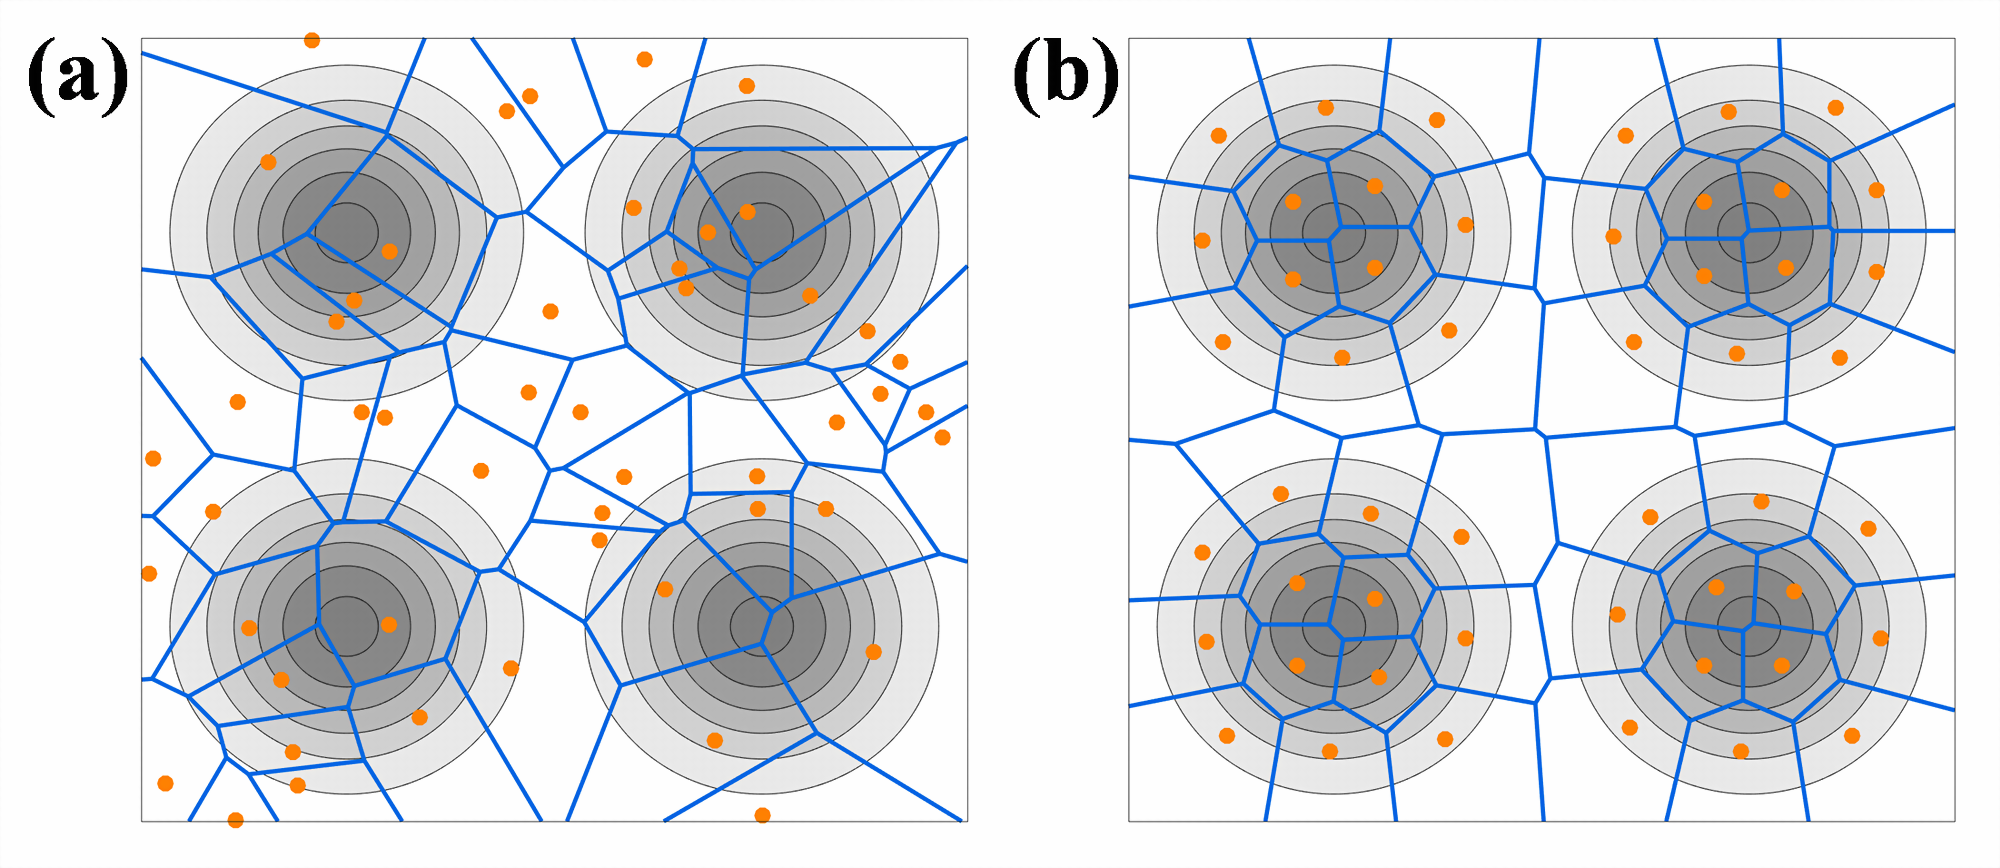
\includegraphics[width=\textwidth]{./cvt/pics/CVT.pdf}
  \end{center}
  \caption{Schematic illustration of the CVT procedure in a 2D domain, including
  (a) initial random choice of centroids and Voronoi tessellation and centroidal
  Voronoi tessellation generated by the weighted K-Means algorithm. The weight
  function is given by  the linear superposition of 4 Gaussian functions.}
  \label{fig:CVT}
\end{figure}

We also show how the interpolation points are placed and moved in real chemical
systems, i.e. the ammonia-borane (BH$_3$NH$_3$) decomposition reaction process.
Figure~\ref{fig:BH3NH3} (a) shows the electron density of the molecule at the
compressed, equilibrium, and dissociated configurations, respectively, according
to the energy landscape in Fig.~\ref{fig:BH3NH3} (c). We plot the interpolation
points found by the weighted K-Means algorithm in Fig.~\ref{fig:BH3NH3} (b). At
the compressed configuration, all the interpolation points are distributed
evenly around the molecule. As the bond length increases, some interpolation
points are transferred from BH$_3$ to NH$_3$. Finally at the dissociated
configuration, NH$_3$ has more interpolation points around the molecule, since
there are more electrons in NH$_3$ than BH$_3$. Along the decomposition reaction
process, both the transfer of the interpolation points and the potential energy
landscape are smooth with respect to the change of the bond length.


\begin{figure}[htbp]
  \begin{center}
    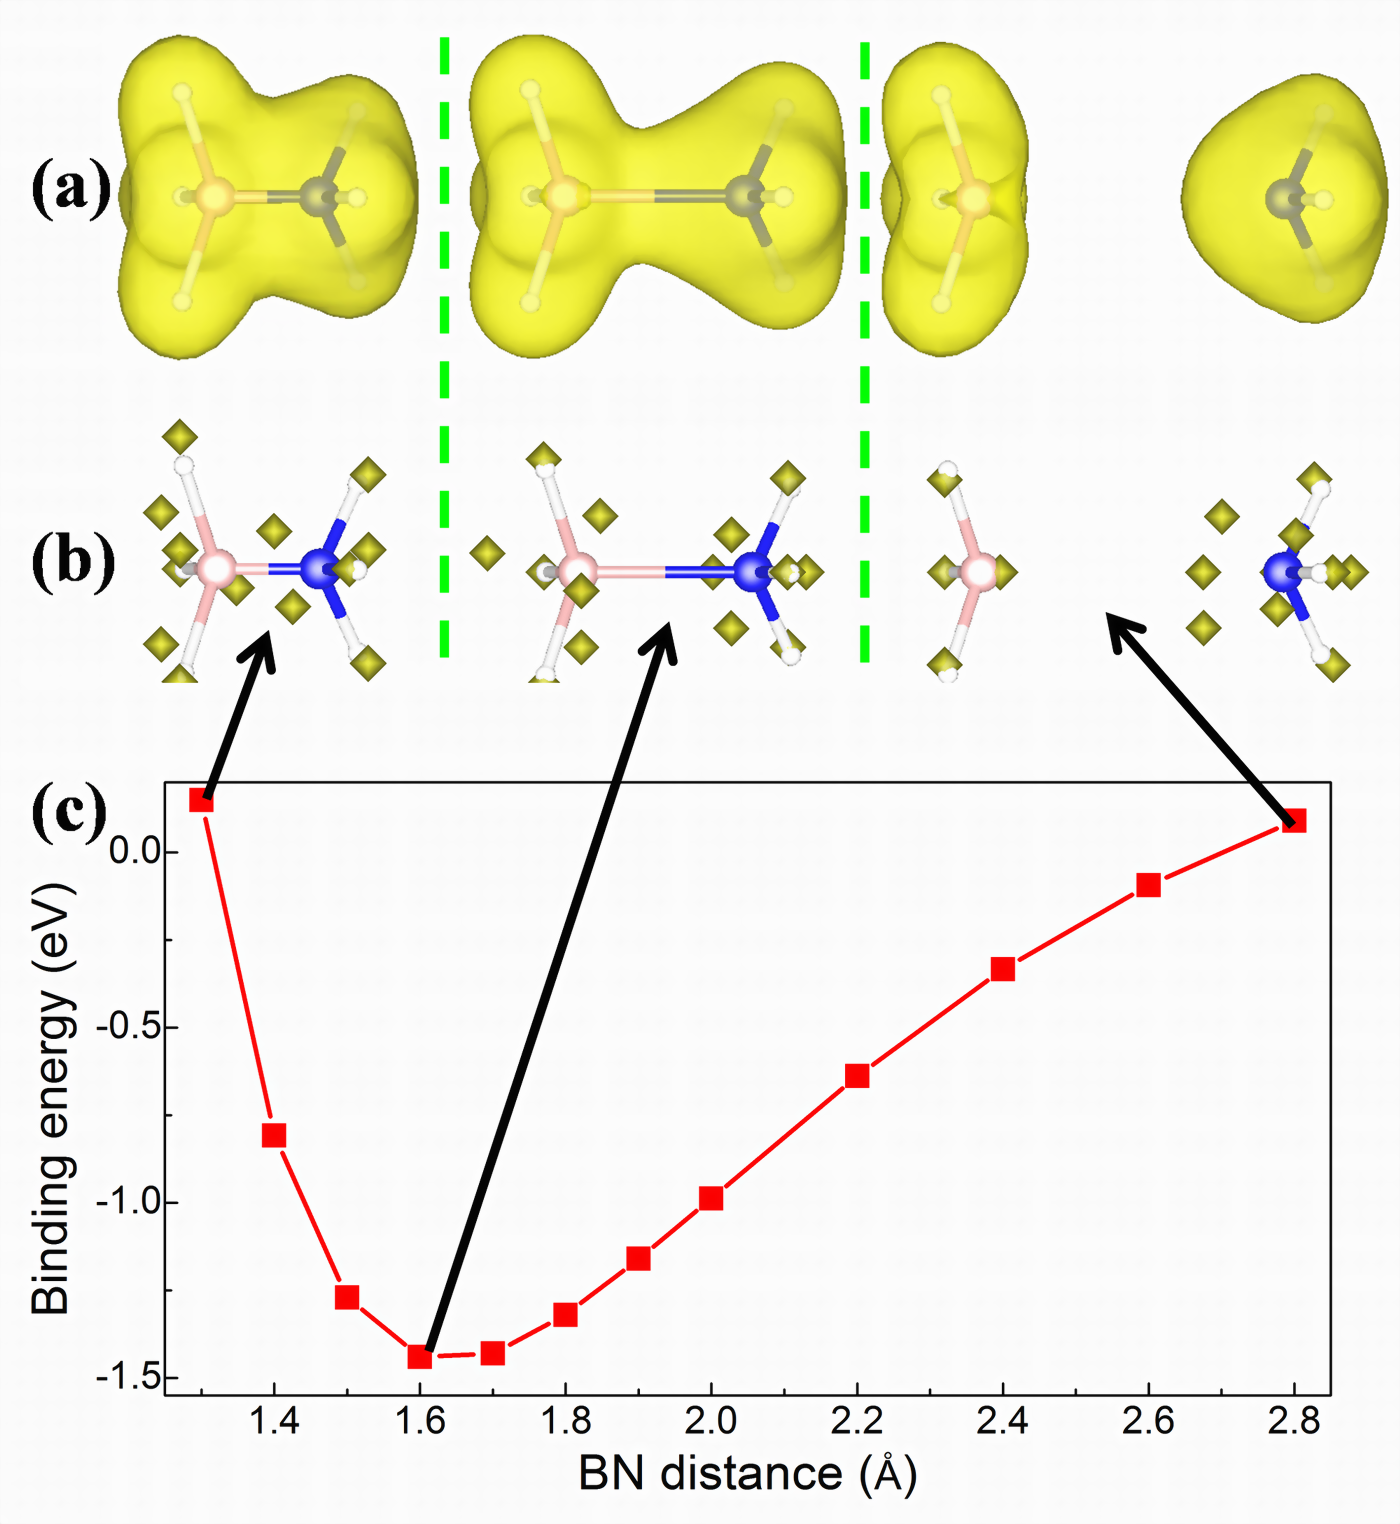
\includegraphics[width=\textwidth]{./cvt/pics/BH3NH3.pdf}
  \end{center}
  \caption{The decomposition reaction process of BH$_3$NH$_3$ computed with
  hybrid functional (HSE06) calculations by using the CVT procedure to select
  interpolation points, including (a) the electron density (yellow isosurfaces),
  (b) the interpolation points (yellow squares) $\{\Brhat_\mu\}_{\mu=1}^{N_
  {\mu}}$ ($N_{\mu}$ = 8) selected from the real space grid points $\{\Br_{i}\}_
  {i=1}^{N_{g}}$ ($N_{g}$ = 100$^3$ and $E_{\text{cut}}$ = 60 Ha) when the BN
  distance respectively is 1.3, 1.7 and 2.8 {\AA} and (c) the binding energy as
  a function of BN distance for BH$_3$NH$_3$ in a 10 {\AA} $\times$ 10 {\AA}
  $\times$ 10 {\AA} box. The white, pink and blue pink balls denote hydrogen,
  boron and nitrogen atoms, respectively.}
  \label{fig:BH3NH3}
\end{figure}